\chapter{Конструкторский раздел}
В данном разделе приводится диаграмма разрабатываемой базы данных. Каждой сущности, описанной в аналитическом разделе, ставится в соответствие таблица, а информация о них соотносится с полями этих таблиц. Рассматриваются разрабатываемые функции, триггеры, а также ролевая модель.

\section{Проектирование базы данных}

В соответствии с таблицей~\ref{tbl:entity} и диаграммой приведенной на рисунке~\ref{fig:chen} в разрабатываемой базе данных выделены следующий таблицы:
\begin{itemize}
    \item[---] user --- таблица пользователей;
    \item[---] book --- таблица книг;
    \item[---] author --- таблица авторов;
    \item[---] book\_author --- таблица-связь книг и авторов;
    \item[---] publisher --- таблица издателей;
    \item[---] bbk --- таблица ББК;
    \item[---] apu --- таблица АПУ;
    \item[---] reservation --- таблица броней;
    \item[---] issuance --- таблица выдач;
    \item[---] favorite --- таблица избранного;
    \item[---] queue --- таблица очередей.
\end{itemize}

В таблицах~\ref{tbl:user} ---~\ref{tbl:queue} определены типы и ограничения для каждого столбца, перечисленных выше таблиц.

В таблице~\ref{tbl:book_author} пара book\_id, author\_id образуют первичный ключ. В таблице~\ref{tbl:favorite} пара user\_id, book\_id образуют первичный ключ.

\begin{table}[H]
    \begin{center}
        \caption{Информация о таблице user}
        \begin{tabular}{|c|c|c|c|}
            \hline
            \textbf{Столбец} & \textbf{Значение} & \textbf{Тип} & \textbf{Ограничение} \\
            \hline
            id & Идентификатор & UUID & Не ноль, первичный ключ \\
            \hline
            surname & Фамилия & Строка & Не ноль \\
            \hline
            name & Имя & Строка & Не ноль \\
            \hline
            second\_name & Отчество & Строка &  \\
            \hline
            phone\_number & Номер телефона & Строка & Не ноль, уникальный \\
            \hline
          	email & Электронная почта & Строка & \\
            \hline
            password & Пароль & Строка & Не ноль \\
            \hline
            role & Роль в системе & Строка & Не ноль \\
            \hline
        \end{tabular}
        \label{tbl:user}
    \end{center}
\end{table}

\begin{table}[H]
    \begin{center}
        \caption{Информация о таблице book}
        \begin{tabular}{|c|p{4cm}|c|p{4cm}|}
            \hline
            \textbf{Столбец} & \textbf{Значение} & \textbf{Тип} & \textbf{Ограничение} \\
            \hline
            id & Идентификатор & UUID & Не ноль, первичный ключ \\
            \hline
            title & Название & Строка & Не ноль \\
            \hline
            annotation & Аннотация & Строка &  \\
            \hline
            publisher\_id & Идентификатор издателя & UUID & Внешний ключ \\
            \hline
            publication\_year & Год публикации & Целое число & Больше нуля, меньше текущего года \\
            \hline
            ISBN & ISBN & Строка &  \\
            \hline
            bbk\_id & Идентификатор ББК & UUID & Не ноль, внешний ключ \\
            \hline
            media\_type & Формат выпуска & Строка &  \\
            \hline
            volume & Объем & Строка &  \\
            \hline
            language & Язык & Строка &  \\
            \hline
            original\_language & Язык оригинала & Строка &  \\
            \hline
            copies & Количество копий & Целое число & Неотрицательный \\
            \hline
            avaliable\_copies & Количество свободных копий & Целое число & Неотрицательно, меньше или равно copies \\
            \hline
        \end{tabular}
    \end{center}
\end{table}

\begin{table}[H]
    \begin{center}
        \caption{Информация о таблице author}
        \begin{tabular}{|c|c|c|c|}
            \hline
            \textbf{Столбец} & \textbf{Значение} & \textbf{Тип} & \textbf{Ограничение} \\
            \hline
            id & Идентификатор & UUID & Не ноль, первичный ключ \\
            \hline
            name & Имя & Строка & Не ноль, уникальный \\
            \hline
        \end{tabular}
    \end{center}
\end{table}

\begin{table}[H]
    \begin{center}
        \caption{Информация о таблице book\_author}
        \begin{tabular}{|c|c|c|c|}
            \hline
            \textbf{Столбец} & \textbf{Значение} & \textbf{Тип} & \textbf{Ограничение} \\
            \hline
            book\_id & Идентификатор книги & UUID & Не ноль, внешний ключ \\
            \hline
            author\_id & Идентификатор автора & UUID & Не ноль, внешний ключ \\
            \hline
        \end{tabular}
        \label{tbl:book_author}
    \end{center}
\end{table}

\begin{table}[H]
    \begin{center}
        \caption{Информация о таблице publisher}
        \begin{tabular}{|c|p{4cm}|c|p{4cm}|}
            \hline
            \textbf{Столбец} & \textbf{Значение} & \textbf{Тип} & \textbf{Ограничение} \\
            \hline
            id & Идентификатор & UUID & Не ноль, первичный ключ \\
            \hline
            name & Название & Строка & Не ноль, уникальный \\
            \hline
            description & Описание & Строка &  \\
            \hline
            email & Электронная почта & Строка &  \\
            \hline
            phone\_number & Номер телефона & Строка &  \\
            \hline
        \end{tabular}
    \end{center}
\end{table}

\begin{table}[H]
    \begin{center}
        \caption{Информация о таблице bbk}
        \begin{tabular}{|c|c|c|c|}
            \hline
            \textbf{Столбец} & \textbf{Значение} & \textbf{Тип} & \textbf{Ограничение} \\
            \hline
            id & Идентификатор & UUID & Не ноль, первичный ключ \\
            \hline
            code & ББК-код & Строка & Не ноль, уникальный \\
            \hline
            description & Расшифровка кода & Строка & Не ноль \\
            \hline
        \end{tabular}
    \end{center}
\end{table}

\begin{table}[H]
    \begin{center}
        \caption{Информация о таблице apu}
        \begin{tabular}{|c|c|c|c|}
            \hline
            \textbf{Столбец} & \textbf{Значение} & \textbf{Тип} & \textbf{Ограничение} \\
            \hline
            id & Идентификатор & UUID & Не ноль, первичный ключ \\
            \hline
            term & Ключевое слово & Строка & Не ноль, уникальный \\
            \hline
            bbk\_id & Идентификатор ББК & UUID & Не ноль, внешний ключ \\
            \hline
        \end{tabular}
    \end{center}
\end{table}

\begin{table}[H]
    \begin{center}
        \caption{Информация о таблице reservation}
        \begin{tabular}{|c|p{4cm}|c|p{4cm}|}
            \hline
            \textbf{Столбец} & \textbf{Значение} & \textbf{Тип} & \textbf{Ограничение} \\
            \hline
            id & Идентификатор & UUID & Не ноль, первичный ключ \\
            \hline
            book\_id & Идентификатор книги & UUID & Не ноль, внешний ключ \\
            \hline
            user\_id & Идентификатор пользователя & UUID & Не ноль, внешний ключ \\
            \hline
            reservation\_date & Дата бронирования & Дата & Не ноль \\
            \hline
            cancel\_date & Дата отмены бронирования & Дата & Не ноль, больше reservation\_date \\
            \hline
        \end{tabular}
    \end{center}
\end{table}

\begin{table}[H]
	\begin{center}
		\caption{Информация о таблице issuance}
		\begin{tabular}{|c|p{4cm}|c|p{4cm}|}
			\hline
			\textbf{Столбец} & \textbf{Значение} & \textbf{Тип} & \textbf{Ограничение} \\
			\hline
			id & Идентификатор & UUID & Не ноль, первичный ключ \\
			\hline
			book\_id & Идентификатор книги & UUID & Не ноль, внешний ключ \\
			\hline
			user\_id & Идентификатор пользователя & UUID & Не ноль, внешний ключ \\
			\hline
			issuance\_date & Дата выдачи & Дата & Не ноль \\
			\hline
			return\_date & Крайняя дата возврата & Дата & Не ноль, больше issuance\_date \\
			\hline
		\end{tabular}
		\label{tbl:favorite}
	\end{center}
\end{table}

\begin{table}[H]
	\begin{center}
		\caption{Информация о таблице favorite}
		\begin{tabular}{|c|c|c|c|}
			\hline
			\textbf{Столбец} & \textbf{Значение} & \textbf{Тип} & \textbf{Ограничение} \\
			\hline
			user\_id & Идентификатор пользователя & UUID & Не ноль \\
			\hline
			book\_id & Идентификатор книги & UUID & Не ноль \\
			\hline
		\end{tabular}
	\end{center}
\end{table}


\begin{table}[H]
    \begin{center}
        \caption{Информация о таблице queue}
        \begin{tabular}{|c|p{4cm}|c|p{4cm}|}
            \hline
            \textbf{Столбец} & \textbf{Значение} & \textbf{Тип} & \textbf{Ограничение} \\
            \hline
            id & Идентификатор & UUID & Не ноль, первичный ключ \\
            \hline
            book\_id & Идентификатор книги & UUID & Не ноль, внешний ключ \\
            \hline
            user\_id & Идентификатор пользователя & UUID & Не ноль, внешний ключ \\
            \hline
            created\_time & Время постановки в очередь & Дата и время & Не ноль \\
            \hline
        \end{tabular}
        \label{tbl:queue}
    \end{center}
\end{table}

\clearpage
На рисунке \ref{fig:bd} изображена диаграмма разрабатываемой базы данных, построенная в соответствии с рассмотренными таблицами.
\begin{figure}[H]
	\centering
	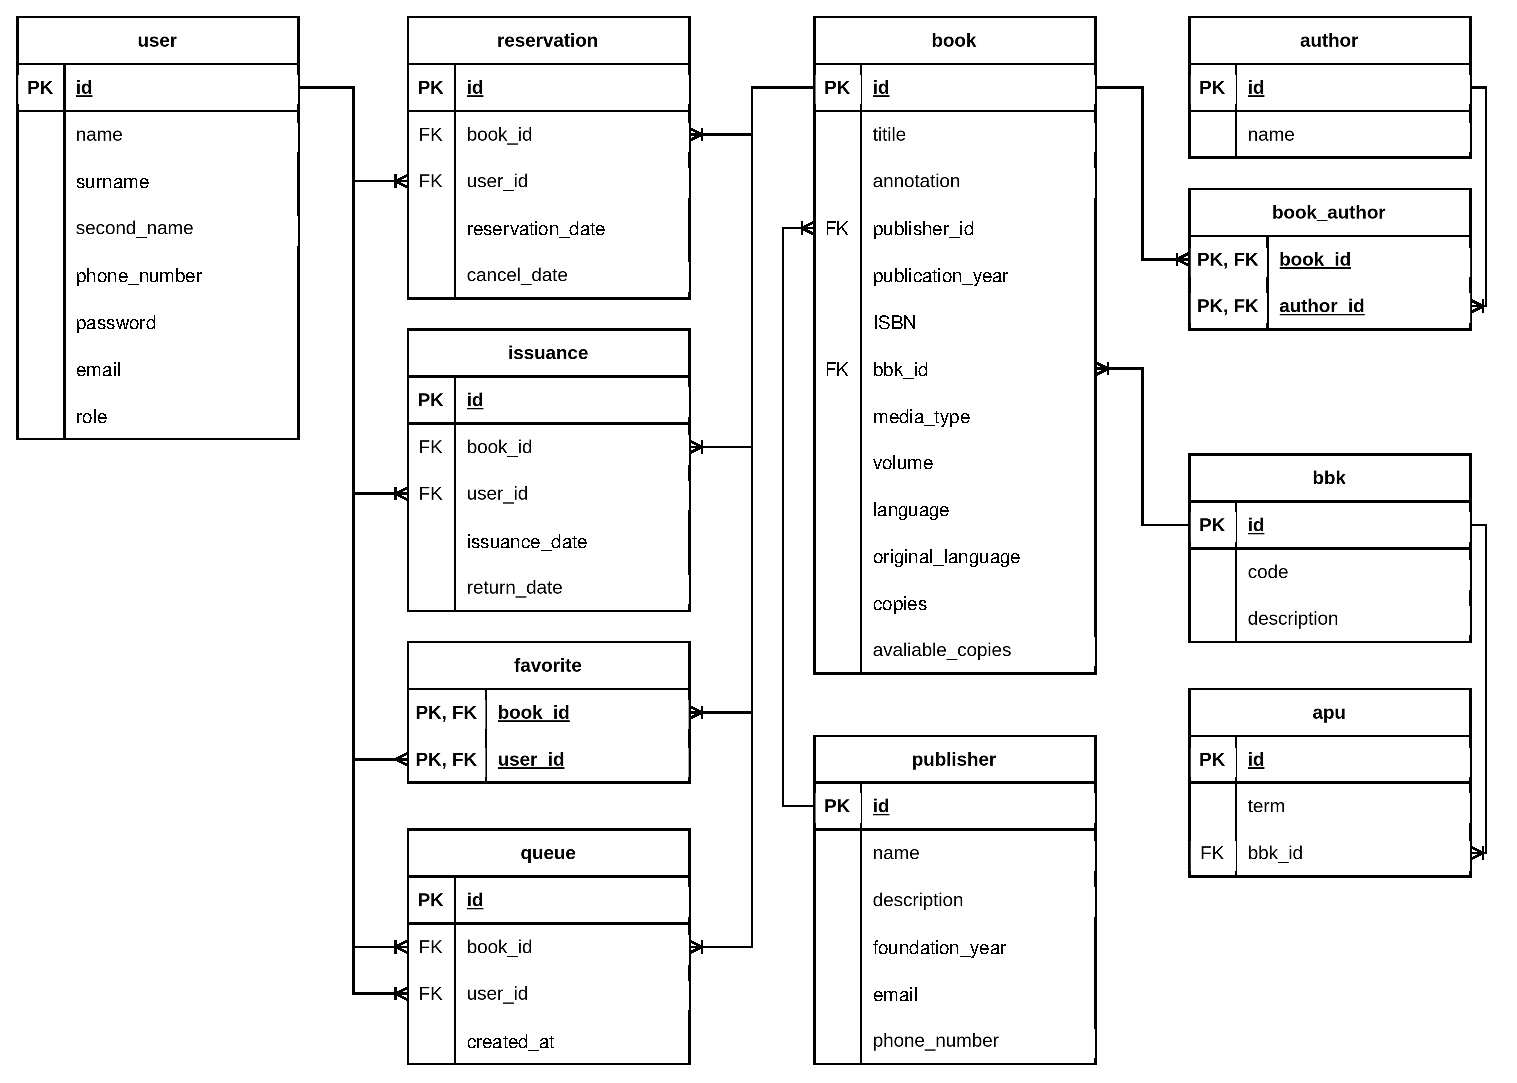
\includegraphics[scale=0.7]{img/DB.eps}
	\caption{Диаграмма разрабатываемой базы данных}
	\label{fig:bd}
\end{figure}

\section{Описание проектируемых функций}
Для корректной работы с базой данных были разработаны функции. Функция process\_book\_return обрабатывает возврат книги после брони или выдачи. Принимает на вход идентификатор обрабатываемой книги. Функция обновляет поле avaliable\_copies в таблице book и создает новую бронь в таблице reservation, если есть пользователь в очереди на эту книгу. Схема алгоритма функции представлена на рисунке~\ref{fig:func_1}.

Функция process\_book\_loan обрабатывает создание брони или выдачи на книгу. Функция генерирует исключение, если avaliable\_copies меньше или равно нулю. Схема алгоритма функции представлена на рисунке~\ref{fig:func_2}.

Функция get\_queue\_number возвращает позицию в очереди пользователя на книгу. Схема алгоритма функции представлена на рисунке~\ref{fig:func_3}.

\begin{figure}[H]
	\centering
	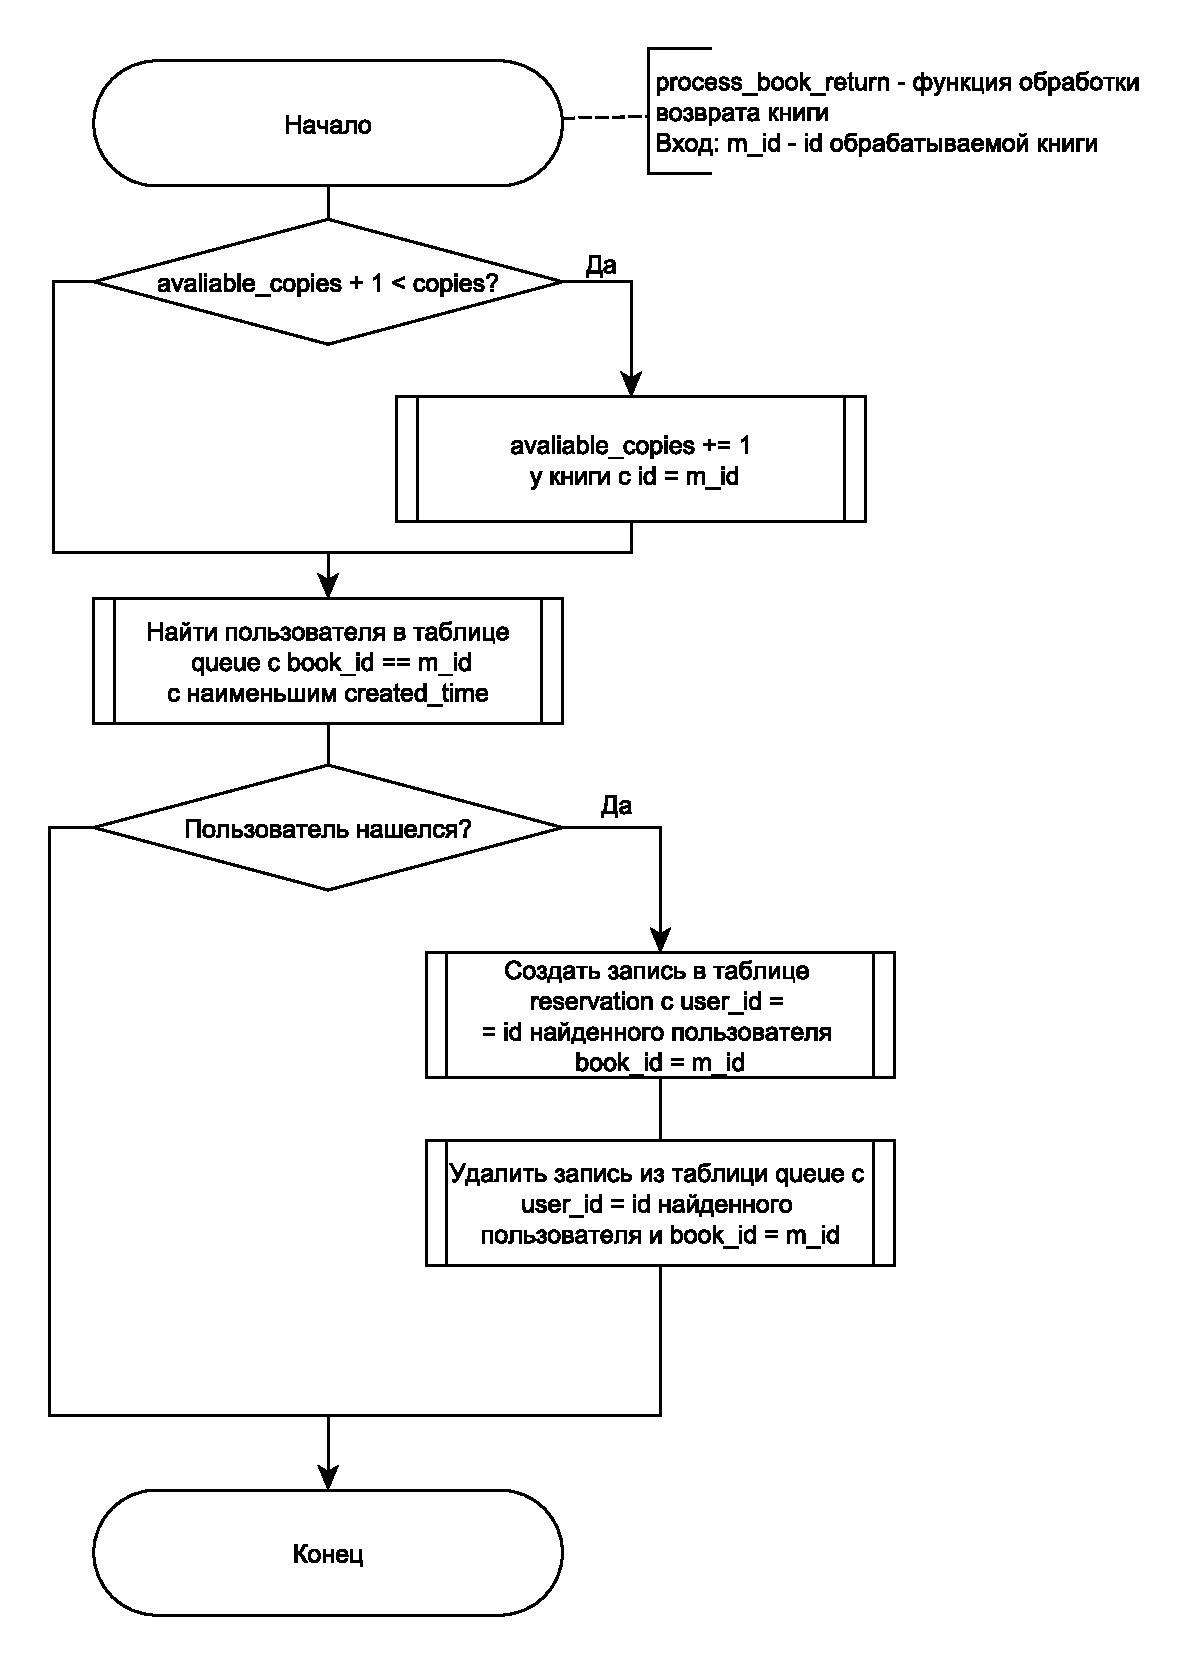
\includegraphics[scale=0.5]{img/func_1.eps}
	\caption{Схема алгоритма функции process\_book\_return}
	\label{fig:func_1}
\end{figure}

\begin{figure}[H]
	\centering
	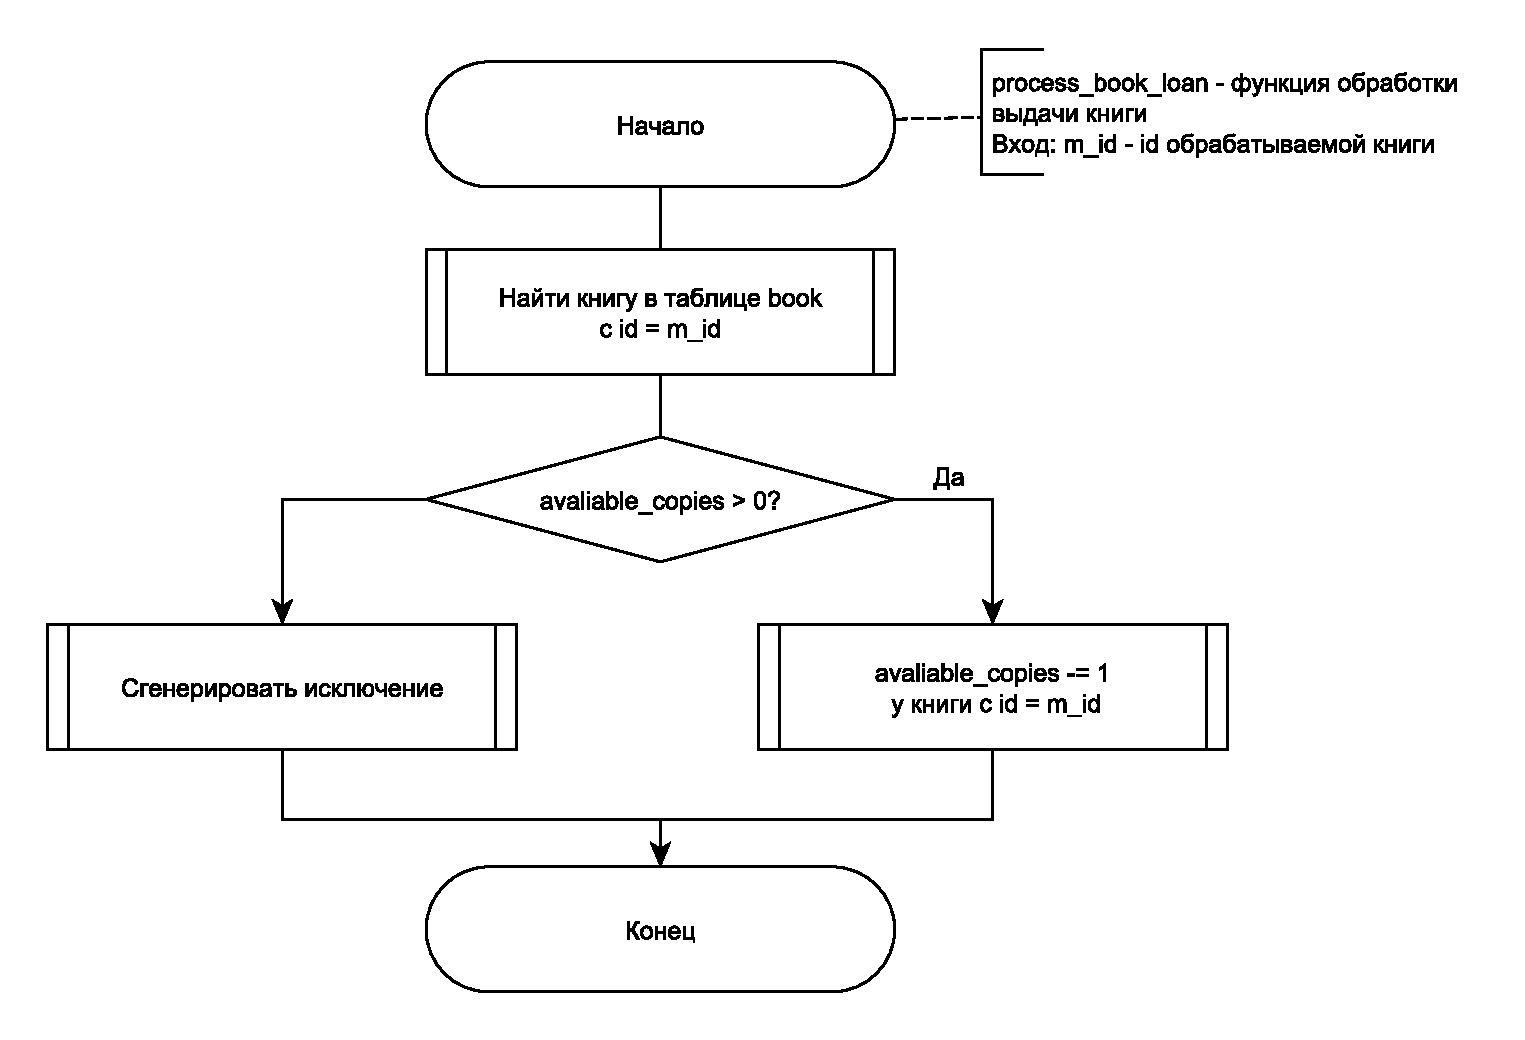
\includegraphics[scale=0.5]{img/func_2.eps}
	\caption{Схема алгоритма функции process\_book\_loan}
	\label{fig:func_2}
\end{figure}

\begin{figure}[H]
	\centering
	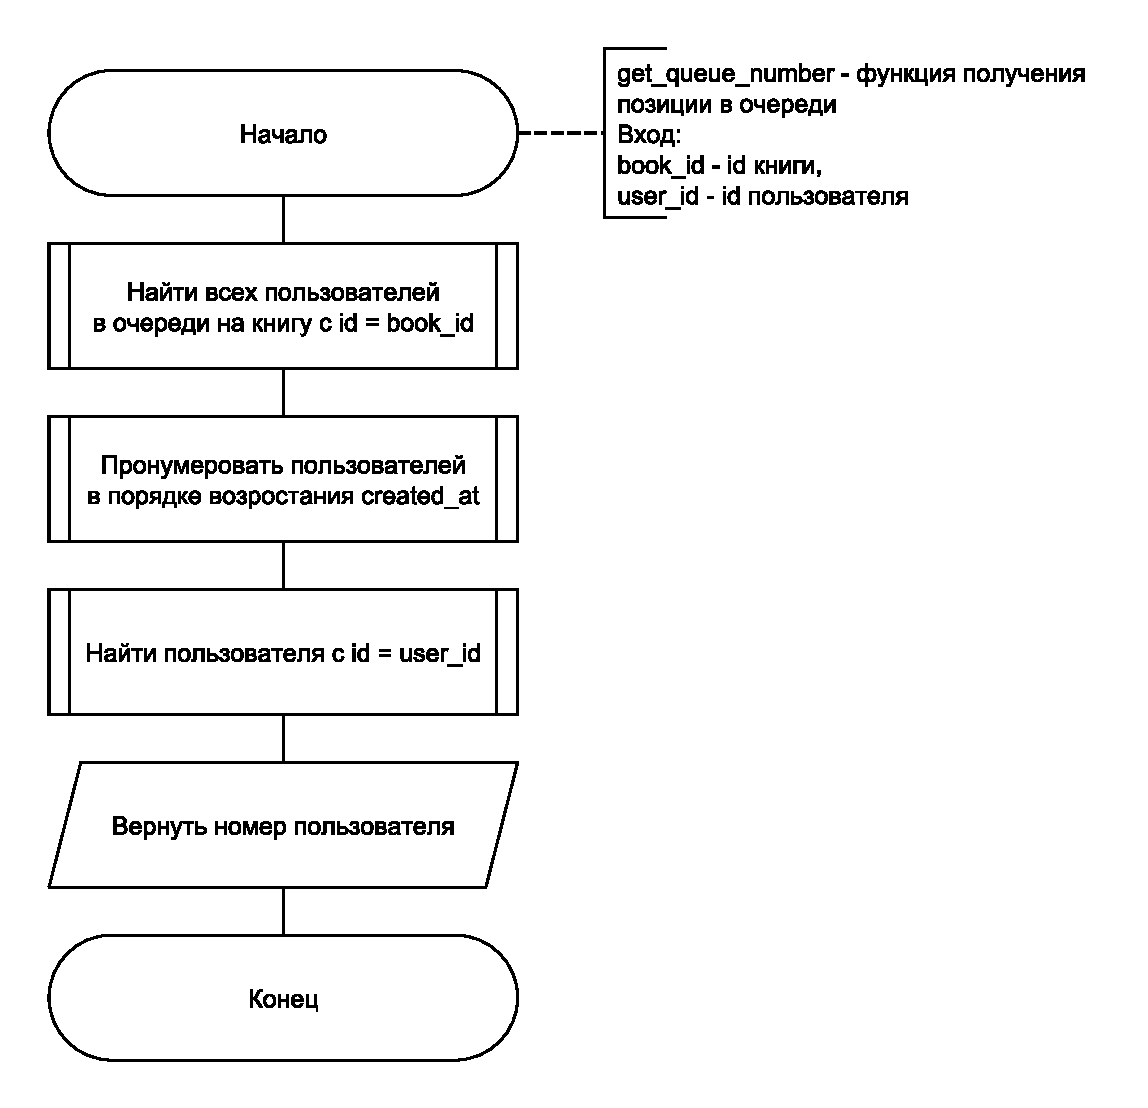
\includegraphics[scale=0.5]{img/func_3.eps}
	\caption{Схема алгоритма функции get\_queue\_number}
	\label{fig:func_3}
\end{figure}


\section{Описание проектируемых триггеров}
Так как поле avaliable\_copies в таблице book зависит как от количества броней, так и от количества выдач книги, были разработаны по два триггера на каждую из таблиц reservation и issuance. При добавлении записи в одну из них вызывается триггер, который в свою очередь вызывает функцию process\_book\_loan. При удалении записи из этих таблиц вызывается триггер, который вызывает функцию process\_book\_return.


\section{Описание ролевой модели}
В аналитическом разделе были описаны четыре категории пользователей, которые могут взаимодействовать с приложением: гость, читатель, библиотекарь, модератор. Для каждой из этих категорий требуется создать роль в базе данных.
\begin{enumerate}
    \item Гость может просматривать таблицы book, author, bbk, apu, book\_author, некоторые столбцы таблицы publisher. Так как гость имеет возможность зарегистрироваться или авторизироваться, то у него должна быть возможность просматривать и добавлять записи в таблицу user;
    \item Читатель может просматривать таблицы book, author, bbk, apu, book\_author, favorite, issuance, user, reservation, некоторые столбцы таблицы publisher. Так как читатель должен иметь возможность получать свой номер в очереди на книгу, то у него должен быть полный доступ на чтение к таблице queue. Также читатель может добавлять и удалять записи в таблицах favorite, reservation, queue;
    \item Библиотекарь может просматривать таблицы book, author, bbk, apu, book\_author, publisher, просматривать и удалять записи из таблицы reservation, просматривать, добавлять и удалять записи в таблице issuance;
    \item Модератор имеет полный доступ ко всем таблицам. 
\end{enumerate}

\textbf{ВЫВОД}

В данном разделе была спроектирована база данных. Описаны все таблицы и их поля, предъявлены ограничения к ним, описаны две разрабатываемые функции и триггеры. Также была разобрана ролевая модель базы данных, описаны ограничения на каждую из четырех ролей.

\clearpage